\begin{aosachapter}{Audacity}{s:audacity}{James Crook}
%% Based on EN-Revision r229

%% Audacity is a popular sound recorder and audio editor.  It is a
%% capable program while still being easy to use.  The majority of users
%% are on Windows but the same Audacity source code compiles to run on
%% Linux and Mac too.
Audacityは、よく知られたサウンドレコーダー/オーディオエディタだ。多機能なプログラムでありながら、使いやすさも維持している。大半のユーザーはWindows上で使っているが、AudacityのソースコードをコンパイルしてLinuxやMacでも使える。

%% Dominic Mazzoni wrote the original version of Audacity in 1999 while
%% he was a research student at Carnegie Mellon University.  Dominic
%% wanted to create a platform on which to develop and debug audio
%% processing algorithms.  The software grew to become useful in its own
%% right in many other ways.  Once Audacity was released as open source
%% software, it attracted other developers.  A small, gradually-changing
%% team of enthusiasts have modified, maintained, tested, updated,
%% written documentation for, helped users with, and translated
%% Audacity's interface into other languages over the years.
Dominic Mazzoniが最初にAudacityを書いたのは1999年のこと。当時の彼はカーネギーメロン大学の研究生で、音響処理アルゴリズムの開発やデバッグに使うプラットフォームを作ろうとしていた。その後このソフトは成長し、当初の目的以外にもいろいろな方面で役立つようになった。Audacityがオープンソースソフトウェアとして公開されると、多くの開発者がそれにひきつけられた。熱心なファンたちが参加し、Audacityの改良や保守、テスト、更新、ドキュメント作成、ユーザーのサポートなどを行うようになった。また、長い年月をかけて、ユーザーインターフェイスも他の言語に翻訳された。

%% One goal is that its user interface should be discoverable:
%% people should be able to sit down without a manual and start using it
%% right away, gradually discovering its features.  This principle has
%% been crucial in giving Audacity greater consistency to the user
%% interface than there otherwise would be.  For a project in which many
%% people have a hand this kind of unifying principle is more important
%% than it might seem at first.
Audacityのひとつの目標は、ユーザーインターフェイスを``発見可能''なものにするということだ。特にマニュアルを読まずともすぐに使い始めることができ、使っていくうちにいろいろな機能を発見できるようになることを目指している。この方針もあり、Audacityは他のソフトに比べてユーザーインターフェイスの一貫性をより重視している。多くの人がかかわるプロジェクトでは、このような統一指針が思いのほか重要となる。

%% It would be good if the architecture of Audacity had a similar guiding
%% principle, a similar kind of discoverability.  The closest we have to
%% that is ``try and be consistent''.  When adding new code, developers try
%% to follow the style and conventions of code nearby.  In practice,
%% though, the Audacity code base is a mix of well-structured and less
%% well-structured code.  Rather than an overall architecture the analogy
%% of a small city is better: there are some impressive buildings but you
%% will also find run-down neighborhoods that are more like a shanty
%% town.
Audacityのアーキテクチャにも同様の指針や発見可能性があればどんなによいことか。それに近いこととして我々が言えるのは``試して、そして合わせよ''ということだ。新しいコードを追加するとき、開発者はその周辺のコードを見てその形式や規約に合わせようとする。しかし実際のところ、Audacityのコードベースには、しっかり構成されたコードとそうでないコードが入り混じっている。全体のアーキテクチャを、小さな都市になぞらえて考えるとわかりやすい。印象的な建造物がいくつかある一方で、そのそばには荒廃した貧民街も見受けられるという具合だ。

%% \begin{aosasect1}{Structure in Audacity}
\begin{aosasect1}{Audacityの構造}

%% Audacity is layered upon several libraries.  While most new
%% programming in Audacity code doesn't require a detailed knowledge of
%% exactly what is going on in these libraries, familiarity with their
%% APIs and what they do is important.  The two most important libraries
%% are PortAudio which provides a low-level audio interface in a
%% cross-platform way, and wxWidgets which provides GUI components in a
%% cross-platform way.
Audacityは、いくつかのライブラリによる階層構造になっている。Audacityのコードに新しいプログラムを追加するときにはこれらのライブラリに関する詳細な知識は不要だが、ライブラリのAPIやその役割に親しんでおくことは大切だ。中でも最も重要なライブラリはPortAudioとwxWidgetsだ。PortAudioはローレベルのオーディオインターフェイスをクロスプラットフォームで提供し、wxWidgetsはGUIコンポーネントを同じくクロスプラットフォームで提供する。

%% When reading Audacity's code,
%% it helps to realize that only a fraction of the code is essential.
%% Libraries contribute a lot of optional features---though people who
%% use those features might not consider them optional.  For example, as
%% well as having its own built-in audio effects, Audacity supports
%% LADSPA (Linux Audio Developer's Simple Plugin API) for dynamically
%% loadable plugin audio effects.  The VAMP API in Audacity does the same
%% thing for plugins that analyze audio.  Without these APIs, Audacity
%% would be less feature-rich, but it does not absolutely depend on these
%% features.
Audacityのコードを読むときには、本質的に不可欠なコードは一部だけであることを知っておけば理解の助けになる。さまざまなオプション機能を提供しているのは各種のライブラリだ---ユーザーはそれをオプション機能だとは考えないかもしれないが。たとえば、組み込みのオーディオエフェクト以外にAudacityはLADSPA (Linux Audio Developer's Simple Plugin API)をサポートしており、オーディオエフェクトのプラグインを動的に読み込むことができる。AudacityのVAMP APIは、オーディオ解析用のプラグインのために同じ仕組みを用意している。これらのAPIがなければAudacityの機能はあまり豊富とはいえなくなるだろうが、プラグインの機能に依存しないものとなる。

%% Other optional libraries used by Audacity are libFLAC, libogg,
%% and libvorbis.  These provide various audio compression formats.  MP3
%% format is catered for by dynamically loading the LAME or FFmpeg
%% library.  Licensing restrictions prevent these very popular
%% compression libraries from being built-in.
Audacityが使うその他のオプションライブラリにはlibFLACやliboggそしてlibvorbisがある。これらは、さまざまなオーディオ圧縮フォーマットに対応する機能を提供する。MP3フォーマットへの対応は、LAMEあるいはFFmpegライブラリを動的に読み込むことで行う。ライセンス上の制約のため、これら主要圧縮フォーマットのライブラリはAudacity本体に組み込むことができない。

%% Licensing is behind some other decisions about Audacity libraries and
%% structure.  For example, support for VST plugins
%% is not built in because of licensing restrictions.
%% We would also like to use the very efficient FFTW
%% fast Fourier transform code in some of our code.  However, we only
%% provide that as an option for people who compile Audacity themselves,
%% and instead fall back to a slightly slower version in our normal
%% builds.  As long as Audacity accepts plugins, it can be and has been
%% argued that Audacity cannot use FFTW\@.  FFTW's authors do not want
%% their code to be available as a general service to arbitrary other
%% code.  So, the architectural decision to support plugins leads to a
%% trade-off in what we can offer.  It makes LADSPA plugins possible but
%% bars us from using FFTW in our pre-built executables.
それ以外にも、ライセンスの影響がAudacityのライブラリや構造にあらわれているところがいくつかある。たとえば、VSTプラグインに対応していないのはライセンスの制約のためだ。また、非常に効率的な高速フーリエ変換ライブラリであるFFTWをいくつかの箇所で使っているが、これはAudacityをソースからコンパイルする人でないと使えない。バイナリ版では、多少速度の落ちる別の実装を使うことになっている。Audacityがプラグインの仕組みを受け付ける限り、AudacityではFFTW\@を使えない。FFTWの作者は、自分のコードを一般的なサービスとして任意のコードで使わせるということを望んでいないのだ。つまり、プラグインをサポートすると決断することで、FFTWを使えないという代償を払うことになる。プラグインをサポートしたおかげでLADSPAプラグインを使えるようになったが、ビルド済みのバイナリ版ではFFTWを使えなくなった。

%% Architecture is also shaped by considerations of how best to use our
%% scarce developer time.  With a small team of developers, we do not
%% have the resources to do, for example, the in-depth analysis of
%% security loopholes that teams working on Firefox and Thunderbird do.
%% However, we do not want Audacity to provide a route to bypass a
%% firewall, so we have a rule not to have TCP/IP connections to or from
%% Audacity at all.  Avoiding TCP/IP cuts out many security concerns.
%% The awareness of our limited resources leads us to better design.  
%% It helps us cut features that would cost us too much in developer 
%% time and focus on what is essential.
アーキテクチャを決める際には、開発者たちの限られた時間をいかにして最大限に生かすかということも検討材料となる。我々開発チームの規模は小さいので、使えるリソースも限られている。たとえばFirefoxやThunderbirdの開発チームがセキュリティホールを詳細に調べるのと同じようなことはできない。しかし我々は、Audacityにファイヤウォールを回避するような抜け道を仕込むつもりはない。そこで、AudacityではTCP/IPコネクションを一切扱わないことに決めた。TCP/IPを切り捨てれば、セキュリティに関して考えるべきことを大幅に減らせる。リソースが限られているのを認識したことで、よりよい設計に向かうことができた。開発者に必要以上の時間をとらせる機能をカットし、より本質的な機能に集中できるようにしたのだ。

%% A similar concern for developers' time applies to scripting languages.
%% We want scripting, but the code implementing the languages does not
%% need to be in Audacity.  It does not make sense to compile copies of
%% each scripting language into Audacity to give users all the choices
%% they could want.\footnote{The one exception to this is the Lisp-based
%% Nyquist language which has been built into Audacity from very early
%% days.  We would like to make it a separate module, bundled with
%% Audacity, but we have not yet had the time to make that change.}
%% We have instead implemented scripting with a single plugin module and a
%% pipe, which we will cover later.
同じく開発者たちの時間を考慮したのが、スクリプト言語の扱いだ。スクリプトでAudacityを操作できるようにしたいが、スクリプト言語を実装するコードはAudacityの中に組み込む必要はない。各言語の処理系をAudacityに組み込んでコンパイルし、ユーザーに好きなものを使わせるというのはあまり意味がない。\footnote{唯一の例外はLispベースの言語Nyquistで、これはAudacityの開発が始まったばかりのころから組み込まれている。できることなら別のモジュールに分割してAudacityにバンドルする形式にしたいところだが、その作業に時間を割く余裕がない。}そのかわりに、スクリプトによる操作はひとつのプラグインモジュールとパイプを使って実装することにした。後ほど説明する。

%% \aosafigure[350pt]{../images/audacity/Layers.eps}{Layers in Audacity}{fig.aud.1}
\aosafigure[350pt]{../images/audacity/Layers.eps}{Audacityの階層}{fig.aud.1}

%% \aosafigref{fig.aud.1} shows some layers and modules in Audacity.  The
%% diagram highlights three important classes within wxWidgets, each of
%% which has a reflection in Audacity.  We're building higher-level
%% abstractions from related lower-level ones.  For example, the
%% BlockFile system is a reflection of and is built on wxWidgets'
%% wxFiles.  It might, at some stage, make sense to split out BlockFiles,
%% ShuttleGUI, and command handling into an intermediate library in their
%% own right.  This would encourage us to make them more general.
\aosafigref{fig.aud.1}は、Audacityのレイヤーとモジュールを図示したものだ。図を見ると3つの重要なクラスがwxWidgets内で強調されており、それぞれに対応するものがAudacityにも用意されている。高レベルの抽象化を、例レベルのクラスに対して行っているのだ。たとえばBlockFileシステムはwxWidgetsのwxFilesに対応するもので、このクラス上に構築されている。おそらく、いずれはBlockFilesやShuttleGUIそしてコマンド処理を仲介ライブラリとして切り出すことになるだろう。そうすれば、より汎用的にできる。

%% Lower down in the diagram is a narrow strip for ``Platform Specific
%% Implementation Layers.'' Both wxWidgets and PortAudio are OS
%% abstraction layers.  Both contain conditional code that chooses
%% between different implementations depending on the target platform.
図の下のほうには``Platform Specific Implementation Layers''という細長い部分がある。wxWidgetsやPortAudioは、どちらもOSを抽象化するレイヤーだ。どちらにも、対象プラットフォームに依存するさまざまな実装にあわせて処理を切り替えるコードが含まれている。

%% The ``Other Supporting Libraries'' category includes a wide collection
%% of libraries.  Interestingly quite a few of these rely on dynamically
%% loaded modules.  Those dynamic modules know nothing of wxWidgets.
``Other Supporting Libraries''のカテゴリに含まれるのは、さまざまなライブラリの集まりだ。興味深いことに、これらの多くは動的に読み込まれたモジュールを信頼している。これらの動的モジュールはwxWidgetsについて何も知らない。

%% On the Windows platform we used to compile Audacity as a single
%% monolithic executable with wxWidgets and Audacity application code in
%% the same executable.  In 2008 we changed over to using a modular
%% structure with wxWidgets as a separate DLL\@.  This is to allow
%% additional optional DLLs to be loaded at run time where those DLLs
%% directly use features of wxWidgets.  Plugins that plug in above the
%% dotted line in the diagram can use wxWidgets.
Windowsプラットフォーム上では、Audacityを単一の一枚岩な実行ファイルとしてコンパイルしていた。つまりwxWidgetsとAudacityアプリケーションが同じ実行ファイルに含まれている状態だ。2008年にこれをモジュラー構造に変更し、wxWidgetsは個別のDLL\@として用意するようにした。これで、さらに別のDLLを実行時に読み込んだときにもそれらのDLLが直接wxWidgetsの機能を使えるようになった。図中の点線より上に組み込むプラグインは、wxWidgetsを使うことができる。

%% The decision to use DLLs for wxWidgets has its downsides.  The
%% distribution is now larger, partly because many unused functions are
%% provided in the DLLs that would previously have been optimized away.
%% Audacity also takes longer to start up because each DLL is loaded
%% separately.  The advantages are considerable.  We expect modules
%% to have similar advantages for us as they do for Apache.  As we see
%% it, modules allow the core of Apache to be very stable while
%% facilitating experimentation, special features and new ideas in the
%% modules.  Modules go a very long way to counteracting the temptation
%% to fork a project to take it in a new direction.  We think it's been a
%% very important architectural change for us.  We're expecting these
%% advantages but have not seen them yet.  Exposing the wxWidgets
%% functions is only a first step and we have more to do to have a
%% flexible modular system.
wxWidgetsをDLL化したことによるマイナス面もある。まず、配布ファイルのサイズが大きくなった。その理由のひとつは、使ってもいない多くの関数がDLLに組み込まれているからである。DLL化する前は、これらは最適化されていた。また、Audacityの起動にやや時間がかかるようになった。各DLLを個別に読み込むためである。しかし、メリットも多い。モジュール化することで、ちょうどApacheのモジュールと同じようなメリットが得られることを期待している。モジュール化したおかげでApache本体は非常に安定するし、その一方で実験的な開発や特殊な機能、新たなアイデアなどはモジュールで試すことができる。モジュールのおかげで、プロジェクトをフォークして別の道を行くという衝動に対抗することができる。モジュール化するという決断は、我々にとって非常に重要なアーキテクチャ変更だったと考えている。これらのメリットが得られるだろうと期待してはいるが、今のところはまだ得られていない。wxWidgetsの機能を公開することは単なるはじめの一歩に過ぎず、我々はより柔軟なモジュラーシステムに向かってさらに進んでいく。

%% The structure of a program like Audacity clearly is not designed up
%% front.  It is something that develops over time.  By and large the
%% architecture we now have works well for us.  We find ourselves
%% fighting the architecture when we try to add features that affect many
%% of the source files.  For example, Audacity currently handles stereo
%% and mono tracks in a special cased way.  If you wanted to modify
%% Audacity to handle surround sound you'd need to make changes in many
%% classes in Audacity.
Audacityのようなプログラムの構造は、前もって明確に設計できるものではない。時間をかけて成長させていくものだ。全体的に見て、現状のアーキテクチャはうまくいっている。ソースファイルの多くの部分に影響する新たな機能を追加するときには、アーキテクチャと対決している気分になる。たとえば、Audacityは現在ステレオとモノラルのトラックをそれぞれ専用の方法で処理している。Audacityを改造してサラウンドサウンドを処理させるようにしようとすれば、Audacity内の多くのクラスに手を入れる必要がある。
\newpage %to keep this sidebar right here.
%% \begin{aosabox}{Going Beyond Stereo: The \code{GetLink} Story}
\begin{aosabox}{ステレオのその先に: \code{GetLink}の物語}

%% Audacity has never had an abstraction for number of channels.  Instead
%% the abstraction it uses is to link audio channels.  There is a
%% function \code{GetLink}that returns the other audio channel in a pair
%% if there are two and that returns NULL if the track is mono.  Code
%% that uses \code{GetLink} typically looks exactly as if it were
%% originally written for mono and later a test of \code{(GetLink() !=
%%   NULL)} used to extend that code to handle stereo.  I'm not sure it
%% was actually written that way, but I suspect it.  There's no looping
%% using \code{GetLink} to iterate through all channels in a linked list.
%% Drawing, mixing, reading and writing all contain a test for the stereo
%% case rather than general code that can work for n channels where n is
%% most likely to be one or two.  To go for the more general code you'd
%% need to make changes at around 100 of these calls to the
%% \code{GetLink} function modifying at least 26 files.
Audacityは、これまでチャンネル数を抽象化したことがなかった。そのかわりに、音声チャンネルに結びつけた抽象化を使っている。\code{GetLink}という関数があり、この関数は、2チャンネルのときはペアのもう一方の音声チャンネルを返し、モノラルのときにはNULLを返す。\code{GetLink}を使うコードは、まるで最初はモノラル用に書いていたものに後から\code{(GetLink() != NULL)}を使ってステレオ処理のコードを継ぎ足したように見える。本当にそうだったのかは不明だが、私はきっとそうだろうと踏んでいる。\code{GetLink}を使って連結リスト内のすべてのチャンネルを反復処理させるといったループはなく、描画やミキシング、そして読み書きのすべてで「ステレオの場合は…」という場合分けが含まれている。もともとのコードが任意のnチャンネルを処理できて、ほとんどの場合はnが1か2になる、というようにはなっていないのだ。より汎用的なコードにしようとおもったら、約100か所にある\code{GetLink}関数の呼び出しに手を入れなければならない。ファイル数にして少なくとも26以上になる。

%% It's easy to search the code to find \code{GetLink} calls and the
%% changes needed are not that complex, so it is not as big a deal to fix
%% this ``problem'' as it might sound at first.  The \code{GetLink} story
%% is not about a structural defect that is hard to fix.  Rather it's
%% illustrative of how a relatively small defect can travel into a lot of
%% code, if allowed to.
\code{GetLink}を呼び出しているところを検索して適切に変更するのはそんなに複雑な作業ではない。この``問題''を修正するのは、最初に感じたほど大がかりな作業ではないだろう。\code{GetLink}の物語は、修正が困難な構造的欠陥に関するものではない。それよりもむしろ、比較的小規模な欠陥がいかにコードを蝕んでいくかを示すものだ。

%% With hindsight it would have been good to make the \code{GetLink}
%% function private and instead provide an iterator to iterate through
%% all channels in a track.  This would have avoided much special case code for
%% stereo, and at the same time made code that uses the
%% list of audio channels agnostic with respect to the list implementation.
今になってみれば、\code{GetLink}関数はprivateにしてそのかわりにイテレータを提供しておいたほうがよかったのだろう。そうすれば、あるトラック内のすべてのチャンネルを順に処理することができる。これでステレオの場合の処理を特別に書くことも防げるし、音声チャンネルのリストを使うコードはリストの実装を知らなくても書けるようになる。

\end{aosabox}

%% The more modular design is likely to drive us towards better hiding of
%% internal structure.  As we define and extend an external API we'll
%% need to look more closely at the functions we're providing.  This will
%% draw our attention to abstractions that we don't want to lock in to an
%% external API.
設計のモジュール化を進めると、内部構造をうまく隠蔽する方向に我々を導いてくれるだろう。外部向けのAPIを定義して拡張することで、アプリケーションが提供する機能について、よりしっかり見つめなければならないことになる。それによって我々は、外部向けAPIにとらわれない抽象化を心がけるようになるだろう。

\end{aosasect1}

%% \begin{aosasect1}{wxWidgets GUI Library}
\begin{aosasect1}{wxWidgets GUIライブラリ}

%% The most significant single library for Audacity user interface
%% programmers is the wxWidgets GUI library, which provides such
%% things as buttons, sliders, check boxes, windows and dialogs.  It provides
%% the most visible cross-platform behavior.  The wxWidgets library has
%% its own string class \code{wxString}, it has cross-platform
%% abstractions for threads, filesystems, and fonts, and a mechanism for
%% localization to other languages, all of which we use.  We advise
%% people new to Audacity development to first download wxWidgets and
%% compile and experiment with some of the samples that come with that
%% library.  wxWidgets is a relatively thin layer on the underlying GUI
%% objects provided by the operating system.
Audacityのユーザーインターフェイスのプログラマーにとって一番重要なライブラリをひとつあげるとすれば、それはwxWidgets GUIライブラリだ。このライブラリは、ボタンやスライダ、チェックボックス、ウィンドウそしてダイアログなどを提供する。つまり、目に見えるクロスプラットフォームな挙動の大半をこのライブラリが提供していることになる。wxWidgetsライブラリには自前の文字列クラス\code{wxString}が用意されており、スレッドやファイルシステムそしてフォントなどをクロスプラットフォームで抽象化する。また他の言語へのローカライズにも対応しており、これらすべての機能をAudacityで使っている。Audacityの開発に新たに参加しようとする人に勧めるのは、まずwxWidgetsをダウンロードしてコンパイルし、付属のサンプルをいくつか試してみることだ。wxWidgetsは、OSが提供するGUIオブジェクトの上に乗る比較的薄めのレイヤーである。

%% To build up complex dialogs wxWidgets provides not only individual
%% widget elements but also sizers that control the elements' sizes
%% and positions.  This is a lot nicer than giving absolute fixed
%% positions to graphical elements.  If the widgets are resized either
%% directly by the user or, say, by using a different font size, the
%% positioning of the elements in the dialogs updates in a very natural
%% way.  Sizers are important for a cross-platform application.  Without
%% them we might have to have custom layouts of dialogs for each
%% platform.
複雑なダイアログを組み立てるために、wxWidgetsでは個々のウィジェットの要素だけでなくサイザー(sizer)も用意している。これは要素のサイズや位置を制御するもので、図形要素に対して固定の座標での位置指定をするよりもずっとよい。ユーザーが直接ウィジェットのサイズ変更したり、フォントサイズを変更したりしても、ダイアログ内の要素の位置は自然に更新される。サイザーは、クロスプラットフォームなアプリケーションにとって重要となる。もしこれがなければ、ダイアログのカスタムレイアウトをプラットフォームごとに用意しなければならなくなるだろう。

%% Often the design for these dialogs is in a resource file that is
%% read by the program.  However in Audacity we exclusively compile
%% dialog designs into the program as a series of calls to wxWidgets
%% functions.  This provides maximum flexibility: that is, dialogs whose
%% exact contents and behavior will be determined by application level
%% code.
ダイアログのデザインをリソースファイルに書き出すこともよくある。このリソースファイルをプログラムから読み込んで使うのだ。しかしAudacityでは、ダイアログの設計はwxWidgetsの関数呼び出しの形でプログラムに埋め込んでいる。これによって最大限の柔軟性を確保している。つまり、ダイアログの正確な内容や振る舞いをアプリケーションレベルのコードで決定できるということだ。

%% You could at one time find places in Audacity where the initial code
%% for creating a GUI had clearly been code-generated using a graphical
%% dialog building tool.  Those tools helped us get a basic design.  Over
%% time the basic code was hacked around to add new features,
%% resulting in many places where new dialogs were created by
%% copying and modifying existing, already hacked-around
%% dialog code.
かつては、AudacityのGUIを作成するコードの中に、グラフィカルなダイアログ作成ツールで自動生成したのが明らかなコードを見かけることもあった。この手のツールは基本的なデザインを作るときには便利だった。時を経てそのコードにも手が入り、新たな機能が追加された。その後新たなダイアログを作るときには、既存のコードをコピーして流用することが多くなった。すでに自動生成結果に手が加えられたダイアログのコードをだ。

%% After a number of years of such development we found that large
%% sections of the Audacity source code, particularly the dialogs for
%% configuring user preferences, consisted of tangled repetitive code.
%% That code, though simple in what it did, was surprisingly hard to
%% follow.  Part of the problem was that the sequence in which dialogs
%% were built up was quite arbitrary: smaller elements were combined into
%% larger ones and eventually into complete dialogs, but the order in
%% which elements were created by the code did not (and did not need to)
%% resemble the order elements were laid out on screen.  The code was
%% also verbose and repetitive.  There was GUI-related code to transfer
%% data from preferences stored on disk to intermediate variables, code
%% to transfer from intermediate variables to the displayed GUI, code to
%% transfer from the displayed GUI to intermediate variables, and code to
%% transfer from intermediate variables to the stored preferences.  There
%% were comments in the code along the lines of \code{//this is a mess},
%% but it was quite some time before anything was done about it.
そんな開発を何年も続けてきた結果、Audacityのソースコードの多く(特に、ユーザーの環境設定用のダイアログまわり)に複雑なコードの重複が目立つようになった。かつてはシンプルだったのかもしれないが、そんなコードを追いかけるのは大変だ。問題のひとつは、ダイアログを組み立てる手順がばらばらだったことだ。小さめの要素を組み合わせて大きな要素を作り、最終的にダイアログが完成するようになっていたが、コードで要素を作成する順番は画面上での要素の配置順と一致していなかった(一致させる必要もなかった)。コードは冗長で、繰り返しも多かった。GUI関連のコードの中には環境設定のデータをディスクから読み出して中間変数に送るものもあったし、中間変数から表示用GUIに送るコードもあった。また、GUIから中間変数にデータを送るコードもあれば、中間変数からディスクに保存するコードもあった。そのコードのそばには「\code{//これはひどい}」とかいうコメントが入っていたが、何か手を付けようとするまでにはかなり時間がかかってしまった。

\end{aosasect1}

%% \begin{aosasect1}{ShuttleGui Layer}
\begin{aosasect1}{ShuttleGuiレイヤー}

%% The solution to untangling all this code was a new class, ShuttleGui,
%% that much reduced the number of lines of code needed to specify a
%% dialog, making the code more readable.  ShuttleGui is an extra layer
%% between the wxWidgets library and Audacity.  Its job is to transfer
%% information between the two.  Here's an example which results in the
%% GUI elements pictured in \aosafigref{fig.aud.2}.
これらのコードのもつれを解決する手段が新たなクラスShuttleGuiだ。これはダイアログの作成に必要なコードの行数を大幅に減らし、コードをより読みやすくする。ShuttleGuiは新たなレイヤーで、wxWidgetsライブラリとAudacityとの間に挟まるものだ。その役割は、wxWidgetsライブラリとAudacityとの間での情報の受け渡しである。例を示そう。これは\aosafigref{fig.aud.2}のようなGUI要素を作成する。

\begin{figure}[h!]
\begin{minipage}[b]{7cm}
\begin{verbatim}
ShuttleGui S;
// GUI Structure
S.StartStatic("Some Title",...);
{
    S.AddButton("Some Button",...);
    S.TieCheckbox("Some Checkbox",...);
}
S.EndStatic();
\end{verbatim}
\end{minipage}
\begin{minipage}[b]{7cm}
% \aosafigure[200pt]{../images/audacity/SomeDialog.eps}{Example Dialog}{fig.aud.2}
\centering
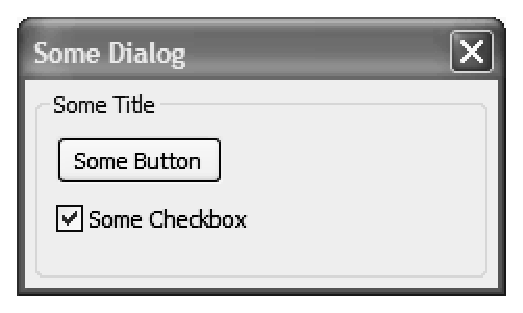
\includegraphics[width={150pt}]{../images/audacity/SomeDialog.eps}
\end{minipage}
%% \caption{Example Dialog}
\caption{ダイアログの例}
\label{fig.aud.2}
\end{figure}

%% This code defines a static box in a dialog and that box contains a
%% button and a checkbox.  The correspondence between the code and the
%% dialog should be clear.  The \code{StartStatic} and \code{EndStatic}
%% are paired calls.  Other similar
%% \code{StartSomething}/\code{EndSomething} pairs, which must match, are
%% used for controlling other aspects of layout of the dialog.  The curly
%% brackets and the indenting that goes with them aren't needed for this
%% to be correct code.  We adopted the convention of adding them in to
%% make the structure and particularly the matching of the paired calls
%% obvious.  It really helps readability in larger examples.
このコードはダイアログ内に静的なボックスを定義し、その中にボタンとチェックボックスをひとつずつ置いている。コードとダイアログの対応は明確だ。\code{StartStatic}と\code{EndStatic}の呼び出しはペアになっている。それ以外にも同様な\code{StartSomething}/\code{EndSomething}のペアがあり、これらは必ずセットで存在しなければならない。これが、ダイアログ上の配置を制御する。波括弧での囲みやその中の字下げは単にコードの見た目だけにかかわるものであり、必須というわけではない。しかし我々は、このように書くよう規約を定めている。コードの構造や\code{StartSomething}/\code{EndSomething}のペアを明確にするためである。コードが巨大になってくると、これが可読性の向上にとても役立つ。

%% The source code shown does not just create the dialog.  The code after
%% the comment ``\code{//GUI Structure}'' can also be used to shuttle
%% data from the dialog out to where the user preferences are stored, and
%% to shuttle data back in.  Previously a lot of the repetitive code came
%% from the need to do this.  Nowadays that code is only written once and
%% is buried within the \code{ShuttleGui} class.
先ほど示したソースコードは、単にダイアログを作るだけではない。コメント``\code{//GUI Structure}''の後に続くコードを使って、ダイアログのデータを設定保存先に送ったり逆にデータを取得したりすることができる。これまでは、同様のことをするためには、同じようなコードを大量に繰り返さねばならなかった。今では、コードを一度だけ書けばあとは\code{ShuttleGui}クラスがうまくやってくれる。

%% There are other extensions to the basic wxWidgets in Audacity.
%% Audacity has its own class for managing toolbars.  Why doesn't it use
%% wxWidget's built in toolbar class?  The reason is historic: Audacity's
%% toolbars were written before wxWidgets provided a toolbar class.
それ以外にもAudacityでは、wxWidgetsの基本機能を拡張するモジュールを使っている。たとえば、Audacityにはツールバーを管理するための自前のクラスがある。なぜwxWidgetの組み込みのツールバークラスを使わなかったのかって?それは、歴史的な理由によるものだ。Audacityのツールバーが書かれたのは、wxWidgetsにツールバークラスが用意されるよりも前のことだったのだ。

\end{aosasect1}

%% \begin{aosasect1}{The TrackPanel}
\begin{aosasect1}{TrackPanel}

%% The main panel in Audacity which displays audio waveforms is the
%% TrackPanel.  This is a custom control drawn by Audacity.  It's made up
%% of components such as smaller panels with track information, a ruler
%% for the timebase, rulers for amplitude, and tracks which may show
%% waveforms, spectra or textual labels.  The tracks can be resized and
%% moved around by dragging.  The tracks containing textual labels make
%% use of our own re-implementation of an editable text box rather than
%% using the built-in text box.  You might think these panels tracks and
%% rulers should each be a wxWidgets component, but they are not.
Audacityのメインパネルで波形を表示しているのがTrackPanelで、これはAudacityのカスタムコントロールだ。このコントロールは、いくつかの小さな部品を組み合わせて作られている。トラック情報を表示するパネルや時間軸のルーラー、振幅のルーラー、そしてトラックの波形やテキストラベルなどだ。トラックのサイズ変更や移動は、マウスのドラッグで行える。トラックにはテキストラベルが含まれているが、これは編集可能なテキストボックスを自前で再実装したものであり、組み込みのテキストボックスではない。これらのパネルやトラック、ルーラーはwxWidgetsのコンポーネントにすべきだと考える人もいるだろう。しかしそのようにはなっていない。

%% \aosafigure{../images/audacity/MainPanelAnnotated.eps}{Audacity Interface with Track Panel Elements Labelled}{fig.aud.3}
\aosafigure{../images/audacity/MainPanelAnnotated.eps}{Audacityのインターフェイスに、Track Panelの要素名を示したもの}{fig.aud.3}

%% The screenshot shown in \aosafigref{fig.aud.3} shows the Audacity user
%% interface.  All the components that have been labelled are custom for
%% Audacity.  As far as wxWidgets is concerned there is one wxWidget
%% component for the TrackPanel.  Audacity code, not wxWidgets, takes
%% care of the positioning and repainting within that.
スクリーンショット\aosafigref{fig.aud.3}にAudacityのユーザーインターフェイスを示す。名前がつけられているコンポーネントはすべて、Audacity用にカスタマイズしたものである。wxWidgetsの観点から見れば、ここにあるwxWidgetのコンポーネントはTrackPanel用のひとつだけだ。その内部の配置や再描画はすべて、wxWidgetではなくAudacity側のコードが面倒を見ている。

%% The way all these components fit together to make the TrackPanel is
%% truly horrible.  (It's the code that's horrible; the end result the
%% user sees looks just fine.)  The GUI and application-specific code is
%% all mixed together, not separated cleanly.  In a good design only our
%% application-specific code should know about left and right audio
%% channels, decibels, muting and soloing.  GUI elements should be
%% application agnostic elements that are reusable in a non-audio
%% application.  Even the purely GUI parts of TrackPanel are a patchwork
%% of special case code with absolute positions and sizes and not enough
%% abstraction.  It would be so much nicer, cleaner and more consistent
%% if these special components were self-contained GUI elements and if
%% they used sizers with the same kinds of interface as wxWidgets uses.
これらのコンポーネントをうまく取りまとめてTrackPanelを作るのは、本当に恐ろしいことだ(恐ろしいのはあくまでもコードのことであって、実際にユーザーが使う完成品はよくできているけどね)。GUIとアプリケーションのコードが入り混じっていて、きれいに分離できていない。きちんと設計するなら、アプリケーションのコードだけが左右のオーディオチャンネルやそのデシベル、ミュート、ソロなどの設定を関知するべきだ。GUIの要素がそれらを関知しているようではいけない。GUIの要素はオーディオ関連以外のアプリケーションでも再利用可能でなければならない。TrackPanel上の部品は、純粋なGUIでさえもつぎはぎだらけのコードになっている。絶対位置やサイズによる場合分けが含まれており、十分に抽象化できていない。これらのコンポーネントが自身でGUI要素を内包してwxWidgetsのsizerのようなインターフェイスを使っていれば、どんなにきれいで一貫性のあるコードになるだろう。

%% To get to such a TrackPanel we'd need a new sizer for wxWidgets that
%% can move and resize tracks or, indeed, any other widget.  wxWidgets
%% sizers aren't yet that flexible.  As a spin off benefit we could use
%% that sizer elsewhere.  We could use it in the toolbars that hold the
%% buttons, making it easy to customize the order of buttons within a
%% toolbar by dragging.
TrackPanelをそんなふうに改良するために、トラックやその他のウィジェットの移動やサイズ変更を行うwxWidgets用の新たなsizerが必要となった。wxWidgetsのsizerは、それを満たすほど柔軟ではない。新たにsizerを作ったおかげで、それを他の部分でも使えるようになった。我々はツールバー上に保持するボタンにもこれを使い、ツールバー上のボタンの並べ替えをドラッグで簡単にできるようにした。

%% Some exploratory work has been done in creating and using such sizers,
%% but not enough.  Some experiments with making the GUI components fully
%% fledged wxWidgets ran into a problem: doing so reduces our control
%% over repainting of the widgets, resulting in flicker when resizing and
%% moving components.  We would need to
%% extensively modify wxWidgets to achieve flicker-free repainting, and
%% better separate the resizing steps from the repainting steps.
新たなsizerを作るために事前調査を行ったが、調査が足りなかったようだ。GUIコンポーネントをwxWidgetsから完全に独立させようとする試みたが、問題が発生した。ウィジェットの再描画がうまく制御できなくなり、コンポーネントのサイズを変更したり移動させたりするとちらつきが発生するようになったのだ。wxWidgetsをベースにして拡張することで再描画時のちらつきを解決し、サイズ変更の処理と再描画の処理をうまく分離させる必要があった。

%% A second reason to be wary of this approach for the TrackPanel is that
%% we already know wxWidgets start running very slowly when there are
%% large numbers of widgets.  This is mostly outside of wxWidget's
%% control.  Each wxWidget, button, and text entry box uses a
%% resource from the windowing system. Each has a handle to access it.
%% Processing large numbers of these takes time.  Processing is slow even
%% when the majority of widgets are hidden or off screen.  We want to be
%% able to use many small widgets on our tracks.
TrackPanelをこの方式で改良するのを躊躇したもうひとつの理由は、ウィジェット数が増えるとwxWidgetsの起動に時間がかかることを既に我々が知っていたからだ。これは、wxWidgetsからはあまり手の施しようのない問題だ。個々のwxWidgetやボタン、テキスト入力ボックスはそれぞれウィンドウシステムのリソースを使っている。そして、個々のリソースは、アクセスするためのハンドルを持っている。多数のハンドルを処理するのには時間がかかる。たとえ大半のウィジェットが非表示あるいはスクリーンの外部にある場合であっても処理が遅くなることは変わらない。我々は、小さなウィジェットを大量に使うつもりだったのだ。

%% The best solution is to use a flyweight pattern, lightweight
%% widgets that we draw ourselves, which do not have corresponding
%% objects that consume windowing system resources or handles.  We would
%% use a structure like wxWidgets's sizers and component widgets, and
%% give the components a similar API but not actually derive from
%% wxWidgets classes.  We'd be refactoring our existing TrackPanel code
%% so that its structure became a lot clearer.  If this were an easy
%% solution it would already have been done, but diverging opinions about
%% exactly what we want to end up with derailed an earlier attempt.
%% Generalizing our current ad hoc approach would take significant design
%% work and coding.  There is a great temptation to leave complex code
%% that already works well enough alone.
最もよい解決策はFlyweightパターンを採用することだ。軽量なウィジェットが自分自身の描画を担当し、対応するオブジェクトを持たないようにすれば、ウィンドウシステムのリソースやハンドルを消費せずに済む。我々はwxWidgetsのsizerやコンポーネントウィジェットと同様の構造を使い、同様のAPIを提供するようにした。しかしそれはwxWidgetsのクラス群を派生させたものではない。我々は既存のTrackPanelのコードをリファクタリングでよりきれいな構造にした。もしこれが簡単な解決法なら既にそうしていただろうが、自分たちがいったい何を求めているのかについての議論が発散した結果、初期の試みから脱線してしまった。現在のアドホックな方式を一般化するには、大変な設計作業とコーディングが必要となる。複雑ではあるけれども今きちんと動いているコードをそのまま残しておきたいという強い誘惑にもかられた。

\end{aosasect1}

%% \begin{aosasect1}{PortAudio Library: Recording and Playback}
\begin{aosasect1}{PortAudioライブラリ: 録音と再生}

%% PortAudio is the audio library that gives Audacity the ability to play
%% and record audio in a cross-platform way.  Without it Audacity would
%% not be able to use the sound card of the device it's running on.
%% PortAudio provides the ring
%% buffers, sample rate conversion when playing/recording and, crucially,
%% provides an API that hides the differences between audio on Mac, Linux
%% and Windows.  Within PortAudio there are alternative implementation
%% files to support this API for each platform.
PortAudioはオーディオライブラリで、Audacityはこれを使って、録音と再生をクロスプラットフォームな方法で提供している。このライブラリがなければ、Audacityは実行環境のサウンドカードを使うことができないだろう。PortAudioが提供する機能にはリングバッファや録音・再生時のサンプルレート変換などがある。重要なのは、そのAPIによってMacやLinuxそしてWindowsにおけるオーディオ処理の差異を隠ぺいできるということだ。PortAudioの内部には、各プラットフォームでAPIに対応するための実装ファイルが別々に用意されている。

%% I've never needed to dig into PortAudio to follow what happens inside.
%% It is, however, useful to know how we interface with PortAudio.
%% Audacity accepts data packets from PortAudio (recording) and sends
%% packets to PortAudio (playback).  It's worth looking at
%% exactly how the sending and
%% receiving happens, and how it fits in with reading and writing to disk
%% and updates to the screen.
私はこれまで、PortAudioの内部に立ち入って何をしているのか追いかける必要などなかった。しかし、AudacityとPortAudioの間でどのようなやりとりをしているかを知っておくと便利だ。Audacityは、PortAudioからデータのパケットを受信(録音)したり、逆にパケットをPortAudioに送信(再生)したりする。送信や受信が実際のところどのように行われているのか、そしてそれがディスクへの読み書きや描画の更新とどのようにつながっているのか。そのあたりは見る価値があるだろう。

%% Several different processes are going on at the same time.  Some
%% happen frequently, transfer small amounts of data, and must be
%% responded to quickly.  Others happen less frequently, transfer larger
%% quantities of data, and the exact timing of when they happen is less
%% critical.  This is an impedance mismatch between the processes,
%% and buffers are used to accommodate it.  A second part of the picture is
%% that we are dealing with audio devices, hard drives,
%% and the screen.  We don't go down to the wire and so have to work with
%% the APIs we're given.  Whilst we would like each of our processes to
%% look similar, for example to have each running from a wxThread, we
%% don't have that luxury (\aosafigref{fig.aud.4}).
いくつかの異なる処理が、同時に発生する。頻繁に発生し、少量のデータをやりとりし、高速な反応を要するものがあれば、あまり頻繁には発生しないが大量のデータをやりとりしなければならないものもある。こちらについては処理がいつ発生するかはそれほど重要ではない。ここに、処理の内容とその対応に使うバッファとの間のインピーダンスミスマッチが発生する。もうひとつ見る価値があるのは、オーディオデバイスやハードディスクそして表示画面などを扱う部分だ。末端まで必死になって追いかけるつもりはなく、与えられたAPIを使って作業をすることになる。各プロセスを同じように見て、たとえばすべてwxThreadから立ち上げるようにしたいものだが、そのような贅沢はできない(\aosafigref{fig.aud.4})。

%% \aosafigureTop[325pt]{../images/audacity/Buffers.eps}{Threads and Buffers in Playback and Recording}{fig.aud.4}
\aosafigureTop[325pt]{../images/audacity/Buffers.eps}{録音・再生時のスレッドとバッファ}{fig.aud.4}

%% One audio thread is started by PortAudio code and interacts directly
%% with the audio device.  This is what drives recording or playback.
%% This thread has to be responsive or packets will get lost.  The
%% thread, under the control of PortAudio code, calls
%% \code{audacityAudioCallback} which, when recording, adds newly arrived
%% small packets to a larger (five second) capture buffer.  When playing
%% back it takes small chunks off a five second playback buffer.  The
%% PortAudio library knows nothing about wxWidgets and so this thread
%% created by PortAudio is a pthread.
ひとつのオーディオスレッドをPortAudioのコードが立ち上げ、それが直接オーディオデバイスとやりとりする。これは、録音や再生を行うものだ。このスレッドは反応が速いものでなければならず、そうでないとパケットを失ってしまう。PortAudioのコードの配下にあるスレッドが\code{audacityAudioCallback}を呼び、録音時には、新たに受け取った小さなパケットを大きめ(5秒)のキャプチャバッファに追加する。再生時には、5秒間の再生バッファから小さな塊を取り出す。PortAudioライブラリはwxWidgetsについては一切知らない。そのため、PortAudioが作ったこのスレッドはpthreadである。

%% A second thread is started by code in Audacity's class AudioIO\@.  When
%% recording, AudioIO takes the data from the capture buffer and appends
%% it to Audacity's tracks so that it will eventually get displayed.
%% Additionally, when enough data has been added, AudioIO writes the data
%% to disk.  This same thread also does the disk reads for audio
%% playback.  The function \code{AudioIO::FillBuffers} is the key
%% function here and depending on the settings of some Boolean variables,
%% handles both recording and playback in the one function.  It's
%% important that the one function handle both directions.  Both the
%% recording and playback parts are used at the same time when doing
%% ``software play through,'' where you overdub what was previously
%% recorded.  In the AudioIO thread we are totally at the mercy of the
%% operating system's disk IO\@.  We may stall for an unknown length of
%% time reading or writing to a disk.  We could not do those reads or
%% writes in \code{audacityAudioCallback} because of the need to be
%% responsive there.
第二のスレッドを立ち上げるのは、AudacityのAudioIO\@クラスだ。録音の際に、AudioIOがデータをキャプチャバッファから受け取り、それをAudacityのトラックに追加して表示させる。さらに、十分な量のデータが追加された時点で、AudioIOがデータをディスクに書き込む。このスレッドは、再生時のディスクからの読み込みも行う。ここで鍵となるのが関数\code{AudioIO::FillBuffers}といくつかのBoolean変数の設定で、録音と再生をこのひとつの関数で行う。重要なのは、このひとつの関数で双方向の処理をしているということだ。録音部と再生部を同時に使うことがある。``software play through''で、以前に録音された内容に対する多重録音を行うときだ。AudioIOのスレッド内では、完全にOSのディスクIO\@にしばられた状態となり、ディスクの読み書きでしばらく待たされることもあるかもしれない。これらの読み書きを\code{audacityAudioCallback}で行うことはできない。この関数は高速な反応を要求されるからである。

%% Communication between these two threads happens via shared variables.
%% Because we control which threads are writing to these variables and
%% when, we avoid the need for more expensive mutexes.
これらふたつのスレッド間の通信は、共有変数を使って行う。どちらの変数がいつ書き込みを行っているのかを制御できているので、ミューテックスを使うようなぜいたくは不要だ。

\pagebreak

%% In both playback and recording, there is an additional requirement:
%% Audacity also needs to update the GUI\@.  This is the least time
%% critical operation.  The update happens in the main GUI thread and is
%% due to a periodic timer that ticks twenty times a second.  This
%% timer's tick causes \code{TrackPanel::OnTimer} to be called, and if
%% updates to the GUI are found to be needed, they are applied.  This
%% main GUI thread is created within wxWidgets rather than by our own
%% code.  It is special in that other threads cannot directly update the
%% GUI\@.  Using a timer to get the GUI thread to check if it needs to
%% update the screen allows us to reduce the number of repaints to a
%% level that is acceptable for a responsive display, and not make too
%% heavy demands on processor time for displaying.
再生と録音の両方で、さらにもうひとつの要件がある。AudacityはGUI\@も更新しなければならないということだ。これは、最もタイムクリティカルでない処理である。描画の更新はメインのGUIスレッドで行われ、1秒間に20回発生する定期的なタイマーで実行される。このタイマーが\code{TrackPanel::OnTimer}を呼び出し、GUIの更新が必要な場所が見つかれば更新する。メインのGUIスレッドは、我々のコードではなくwxWidgetsの中から立ち上げる。他のスレッドからは、直接GUI\@を更新することはできない。タイマーを使ってGUIスレッドを取得し、画面の更新が必要かどうかを調べる。そうすることで、再描画の回数を減らしながらも許容できるレベルの反応を保つ。また、そうすることで、表示用にあまりプロセッサタイムを要求しすぎないようにしている。

%% Is it good design to have an audio device thread, a buffer/disk thread
%% and a GUI thread with periodic timer to handle these audio data
%% transfers?  It is somewhat ad hoc to have these three different
%% threads that are not based on a single abstract base class.  However,
%% the ad-hockery is largely dictated by the libraries we use.  PortAudio
%% expects to create a thread itself.  The wxWidgets framework
%% automatically has a GUI thread.  Our need for a buffer filling thread
%% is dictated by our need to fix the impedance mismatch between the
%% frequent small packets of the audio device thread and the less
%% frequent larger packets of the disk drive.  There is very clear
%% benefit in using these libraries.  The cost in using the libraries is
%% that we end up using the abstractions they provide.  As a result we
%% copy data in memory from one place to another more than is strictly
%% necessary.  In fast data switches I've worked on, I've seen extremely
%% efficient code for handling these kinds of impedance mismatches
%% that is interrupt driven and does not use threads at all.  Pointers to
%% buffers are passed around rather than copying data.  You can only do
%% that if the libraries you are using are designed with a richer buffer
%% abstraction.  Using the existing interfaces, we're forced to use
%% threads and we're forced to copy data.
オーディオデバイス用のスレッドとバッファ/ディスク用のスレッド、そして定期的なタイマーを持つGUIスレッドの三つを使ってオーディオデータのやりとりをするというのは、よい設計と言えるだろうか?これら三種類のスレッドを単一の抽象基底クラスから派生させないのは、多少アドホックにも感じる。しかし、このアドホック性の要因の多くは、使っているライブラリによるものである。PortAudioは、自分自身でスレッドを作ることを想定している。wxWidgetsフレームワークがGUIスレッドを持っているのは、ごく自然なことだ。バッファを埋めるためのスレッドを要する理由は、オーディオデバイスのスレッドで頻繁に発生する小規模のパケットと、あまり頻繁には発生しないディスクドライブの大規模なパケットとの間のインピーダンスミスマッチを解決するためだ。これらのライブラリを使うことには明確な利点がある。逆に、これらのライブラリを使うことで必要となるコストは、結局は各ライブラリが提供する抽象化を使うことになるということだ。結果的に、メモリ内でのデータのコピーの回数が、最低限必要な回数だけでなくさらに増えてしまっている。私がこれまで関わってきた高速なデータ交換の処理ではもっと効率的なコードを見たことがある。そのコードでは、割り込みなどで発生するこの手のインピーダンスミスマッチに対応するのにスレッドなど使っていなかった。データをコピーするのではなく、バッファへのポインタを渡していたのだ。ただ、そんなことができるのは、使っているライブラリがバッファの抽象化をよりリッチに設計している場合だけである。既存のインターフェイスを使う限りはスレッドを使うことを強いられ、そしてデータのコピーを強いられることになる。

\end{aosasect1}

%% \begin{aosasect1}{BlockFiles}
\begin{aosasect1}{BlockFile}

%% One of the challenges faced by Audacity is supporting insertions and
%% deletions into audio recordings that may be hours long.  Recordings
%% can easily be too long to fit in available RAM\@.  If an audio recording
%% is in a single disk file, inserting audio somewhere near the start of
%% that file could mean moving a lot of data to make way.  Copying that
%% data on disk would be time consuming and mean that Audacity could then
%% not respond rapidly to simple edits.
Audacityが直面する困難のひとつが、録音したオーディオデータへのデータの追加や削除だ。オーディオデータの長さは数時間分になることもある。録音データはどんどん長くなり、利用可能なRAM\@の容量を簡単に突破してしまうだろう。録音データをディスク上に単一のファイルとして管理していたとすると、ファイルの先頭あたりにデータを挿入しようとしたときには大量のデータ移動が発生することになる。ディスク上でのデータのコピーには時間がかかる。つまり、Audacityはちょっとした編集でも長々と待たされるソフトウェアになってしまう。

%% Audacity's solution to this is to divide audio files into many
%% BlockFiles, each of which could be around 1 MB\@.  This is the main
%% reason Audacity has its own audio file format, a master file with the
%% extension \code{.aup}.  It is an XML file which coordinates the various
%% blocks.  Changes near the start of a long audio recording might affect
%% just one block and the master \code{.aup} file.
Audacityがこの問題に対処するために使った方法は、オーディオファイルを多数のBlockFileに分割することだ。個々のファイルの大きさは約1 MB\@となる。これが、Audacityが自前のオーディオファイルフォーマットを採用している主な理由だ。マスターファイルの拡張子は\code{.aup}となる。これはXMLファイルで、このファイルがさまざまなブロックを取りまとめている。長いオーディオデータの先頭近くを変更した場合でも、影響を受けるのはたったひとつのブロックとマスターファイル\code{.aup}だけとなる。

%% BlockFiles balance two conflicting forces.  We can insert and delete
%% audio without excessive copying, and during playback we are guaranteed
%% to get reasonably large chunks of audio with each request to the disk.
%% The smaller the blocks, the more potential disk requests to fetch the
%% same amount of audio data; the larger the blocks, the more copying on
%% insertions and deletions.
BlockFileは、対立する二つの勢力の調和をうまく保っている。挿入や削除の際に必要以上のコピーが発生することもないし、再生時には、ディスクへのリクエストのたびに適度に大きなデータの塊を取得できることが保証されている。ブロックが小さくなればなるほど、同じ量のオーディオデータを取得するために必要なディスクへのリクエストの回数が増え、逆に大きくなればなるほど挿入や削除の際のコピーの量が増える。

%% Audacity's BlockFiles never have internal free space and they never
%% grow beyond the maximum block size.  To keep this true when we insert
%% or delete we may end up copying up to one block's worth of data.  When
%% we don't need a BlockFile anymore we delete it.  The BlockFiles are
%% reference counted so if we delete some audio, the relevant BlockFiles
%% will still hang around to support the undo mechanism until we save.
%% There is never a need to garbage collect free space within
%% Audacity BlockFiles, which we would need to do with an all-in-one-file
%% approach.
AudacityのBlockFileは決して内部に空き領域を持たないし、最大のブロックサイズを超えることもない。このルールを守るため、挿入や削除をするときには最大1ブロックまでのデータのコピーが発生する可能性がある。BlockFileが不要になれば、削除する。BlockFileは参照カウンタで管理されているので、オーディオの一部を削除したとしてもそれに関連するBlockFileはまだ残ったままであり、undoに対応できるようにしている。データを保存するまではその状態になる。AudacityのBlockFileには、空き領域のガベージコレクションはまったく不要だ。我々が対応する必要があるのは、オールインワン型のファイルである。

%% Merging and splitting larger chunks of data is the bread and butter of
%% data management systems, from B-trees to Google's BigTable tablets to
%% the management of unrolled linked lists.  \aosafigref{fig.aud.5} shows
%% what happens in Audacity when removing a span of audio near the start.
大きめのデータのマージや分割こそが、データを管理するシステムの本業である。BツリーからGoogleのBigTableのタブレットやUnrolled linked listの管理まで、それは変わらない。\aosafigref{fig.aud.5}は、Audacityでオーディオの開始位置付近を削除したときに何が起こるのかを示している。

%% \aosafigure[200pt]{../images/audacity/BlocksCombined.eps}{Before deletion, \code{.aup} file and BlockFiles hold the sequence ABCDEFGHIJKLMNO. After deletion of FGHI, two BlockFiles are merged.}{fig.aud.5}
\aosafigure[200pt]{../images/audacity/BlocksCombined.eps}{削除する前は\code{.aup}ファイルとBlockFileが保持するのはABCDEFGHIJKLMNO。FGHIを削除すると、ふたつのBlockFileがマージされる。}{fig.aud.5}

%% BlockFiles aren't just used for the audio itself.  There are also
%% BlockFiles that cache summary information.  If Audacity is asked to
%% display a four hour long recording on screen it is not acceptable for
%% it to process the entire audio each time it redraws the screen.
%% Instead it uses summary information which gives the maximum and
%% minimum audio amplitude over ranges of time.  When zoomed in,
%% Audacity is drawing using actual samples.  When zoomed out,
%% Audacity is drawing using summary information.
BlockFileが扱うのはオーディオそのものだけではない。それ以外にも、サマリ情報をキャッシュするBlockFileもある。Audacityで4時間のオーディオデータを表示するときに、画面の再描画のたびにオーディオ全体を読み直すのは考えられない話だ。そういう場合にサマリ情報を代わりに使う。サマリ情報には、その時間の範囲内での最大音量や最小音量が記録されている。表示をズームインしたときは、実際のデータを使って描画を行い、ズームアウトしたときはサマリ情報をもとに描画を行う。

%% A refinement in the BlockFile system is that the blocks needn't be
%% files created by Audacity.  They can be references to subsections of
%% audio files such as a timespan from audio stored in the \code{.wav} format.
%% A user can create an Audacity project, import audio from a \code{.wav} file
%% and mix a number of tracks whilst only creating BlockFiles for the
%% summary information.  This saves disk space and saves time in copying
%% audio.  All told it is, however, a rather bad idea.  Far too many of
%% our users have removed the original audio \code{.wav} file thinking there
%% will be a complete copy in the Audacity project folder.  That's not so
%% and without the original \code{.wav} file the audio project can no longer be
%% played.  The default in Audacity nowadays is to always copy imported
%% audio, creating new BlockFiles in the process.
BlockFileシステムの特徴のひとつに、各ブロックはAudacityが作ったファイルでなくてもかまわないという点がある。たとえば、\code{.wav}形式で保存されたオーディオファイルの特定の時間範囲を指すこともできる。ユーザーがAudacityプロジェクトを立ち上げて\code{.wav}ファイルからオーディオをインポートしていくつかのトラックをミックスしたとしよう。このときに作られるBlockFileはサマリ情報を格納するものだけだ。そのおかげでディスク容量も抑えられるし、オーディオデータをコピーする時間も節約できる。しかしながら、これはあまり良い考えではない。これまでに、多くのユーザーがインポート後に元の\code{.wav}ファイルを削除してしまっていた。Audacityのプロジェクトフォルダに全部コピーされているものと勘違いしていたのだ。実際はそうではなく、元の\code{.wav}ファイルがなければそのプロジェクトは再生できない。そのため、Audacityの現在のデフォルト設定では、インポートしたオーディオを常にコピーして新しいBlockFileを作るようにしている。

%% The BlockFile solution ran into problems on Windows systems where
%% having a large number of BlockFiles performed very poorly.  This appeared
%% to be because Windows was much slower handling
%% files when there were many in the same directory, a similar problem to
%% the slowdown with large numbers of widgets.  A later addition was made
%% to use a hierarchy of subdirectories, never with more than a hundred
%% files in each subdirectory.
BlockFile方式が、Windows上で問題となることがあった。Windows上で大量のBlockFileを扱うと、パフォーマンスが非常に劣化したのだ。原因はおそらく、Windowsでは同一ディレクトリ上にある大量のファイルの処理速度に難があったからだろう。同様の問題が、ウィジェットをたくさん使ったときの速度低下という形でもあらわれた。その後、サブディレクトリ階層を使うように変更を加え、ひとつのディレクトリには最大100個までのファイルしか置かないようにした。

%% The main problem with the BlockFile structure is that it is exposed to
%% end users.  We often hear from users who move the \code{.aup} file and don't
%% realize they also need to move the folder containing all the
%% BlockFiles too.  It would be better if Audacity projects were a single
%% file with Audacity taking responsibility for how the space inside the
%% file is used.  If anything this would increase performance rather than
%% reduce it.  The main additional code needed would be for garbage
%% collection.  A simple approach to that would be to copy the blocks to
%% a new file when saving if more than a set percentage of the file were
%% unused.
BlockFileの構造を使うときの最大の問題は、その構造がエンドユーザーに公開されてしまうことだ。よく聞く話だが、\code{.aup}ファイルを別の場所に移したユーザーが、BlockFileを含むフォルダも一緒に移動させなければならないことに気付かないということがある。Audacityのプロジェクトが単一のファイルにまとまっていて、その内部のスペースやファイル内の利用状況を管理できる状態であればよかっただろう。こうすれば、パフォーマンスはどちらかといえば向上するだろう。追加で必要となるコードは、おそらくガベージコレクションであろう。シンプルなアプローチとしては、ファイルのみ使用領域が設定した割合を上回るときにブロックを新しいファイルへコピーするという方法がある。

\end{aosasect1}

%% \begin{aosasect1}{Scripting}
\begin{aosasect1}{スクリプト}

%% Audacity has an experimental plugin that supports multiple scripting
%% languages.  It provides a scripting interface over a named pipe.  The
%% commands exposed via scripting are in a textual format, as are the
%% responses.  As long as the user's scripting language can write text to
%% and read text from a named pipe, the scripting language can drive
%% Audacity.  Audio and other high-volume data does not need to travel on
%% the pipe (\aosafigref{fig.aud.7}).
Audacityには、複数のスクリプト言語に対応する実験的なプラグインが付属している。このプラグインは、名前付きパイプを使ったスクリプトインターフェイスを提供する。スクリプト用に公開されたコマンドはテキスト形式で、同じくコマンドの応答もテキストとなる。つまり、名前付きパイプへのテキストの書き出しや名前付きパイプからのテキストの読み込みに対応しているスクリプト言語ならなんでも、Audacityを動かせるということだ。オーディオそのものなどの大きなデータにパイプ上を行き来させる必要はない(\aosafigref{fig.aud.7})。

%% \aosafigure[75pt]{../images/audacity/Scripting.eps}{Scripting Plugin Provides Scripting Over a Named Pipe}{fig.aud.7}
\aosafigure[75pt]{../images/audacity/Scripting.eps}{スクリプトプラグインが、名前付きパイプを使ったスクリプト処理機能を提供する}{fig.aud.7}

%% The plugin itself knows nothing about the content of the text traffic
%% that it carries. It is only responsible for conveying it. The plugin
%% interface (or rudimentary extension point) used by the scripting
%% plugin to plug in to Audacity already exposes Audacity commands in
%% textual format.  So, the scripting plugin is small, its main content
%% being code for the pipe.
プラグイン自身は、自分が運ぶテキストの内容については何も知らない。単にそれを運ぶだけだ。スクリプトプラグインが使うプラグインインターフェイス(あるいは原始的な拡張ポイント)は、Audacity側でテキスト形式のコマンドとして公開されている。そのため、スクリプトプラグインは小さなプラグインで、コードの大部分はパイプを扱う処理である。

%% Unfortunately a pipe introduces similar security risks to having a
%% TCP/IP connection---and we've ruled out TCP/IP connections for
%% Audacity on security grounds.  To reduce that risk the plugin is an
%% optional DLL\@.  You have to make a deliberate decision to obtain and
%% use it and it comes with a health/security warning.
残念ながら、パイプを使うということはTCP/IP接続を扱うのと同じセキュリティリスクを負うことになる---セキュリティを考慮してAudacityではTCP/IP接続を扱わないことに決めている。リスクを少しでも下げるために、このプラグインはオプションのDLL\@としている。これを取得して使う前には熟考が必要だ。また、このプラグインを使うときにはセキュリティに関する警告が出る。

%% After the scripting feature had already been started, a suggestion
%% surfaced in the feature requests page of our wiki that we should
%% consider using KDE's D-Bus standard to provide an inter-process call
%% mechanism using TCP/IP\@.  We'd already started going down a different
%% route but it still might make sense to adapt the interface we've ended
%% up with to support D-Bus.
スクリプトの機能を公開した後で、Wikiの機能追加リクエストのページでこんな提案を受けた。KDEのD-Busを使えばTCP/IP\@によるプロセス間通信機能を提供できるのではないか、というものだ。既に別のやりかたで始めたところではあるが、最終的にD-Busをサポートするようになる可能性も残っている。

%% \begin{aosabox}{Origins of Scripting Code}
\begin{aosabox}{スクリプト機能のはじまり}

%% The scripting feature grew from an enthusiast's adaptation of Audacity
%% for a particular need that was heading in the direction of being a
%% fork.  These features, together called CleanSpeech, provide for mp3
%% conversion of sermons.  CleanSpeech adds new effects such as truncate
%% silence---the effect finds and cuts out long silences in audio---and
%% the ability to apply a fixed sequence of existing noise removal
%% effects, normalization and mp3 conversion to a whole batch of audio
%% recordings.  We wanted some of the excellent functionality in this,
%% but the way it was written was too special case for Audacity.
%% Bringing it into mainstream Audacity led us to code for a flexible
%% sequence rather than a fixed sequence.  The flexible sequence could
%% use any of the effects via a look-up table for command names and a
%% \code{Shuttle} class to persist the command parameters to a textual
%% format in user preferences.  This feature is called \emph{batch
%% chains}.  Very deliberately we stopped short of adding conditionals
%% or calculation to avoid inventing an ad hoc scripting language.
スクリプト機能ができたきっかけは、あるAudacityファンから提供された機能だった。それはあるニーズを満たすための機能で、当初はAudacityをフォークする方向に向かっていた。その機能はひとまとめにしてCleanSpeechと呼ばれ、教会での説教をmp3に変換するために作られた。CleanSpeechには無音部分の切り詰め---オーディオ内の長い無音部分を探して切り取る---などの新たなエフェクトやノイズ除去効果のある固定シーケンスを適用する機能があり、オーディオの正規化や録音内容のmp3への変換機能などもあった。中にはぜひ取り込みたくなるような素晴らしい機能もあったが、その実装はAudacity内ではかなり特殊なものだった。それをAudacityの本流に取り込むと、固定シーケンスではなく可変シーケンスのコードを書くことになった。可変シーケンスだと、コマンド名と\code{Shuttle}クラスのルックアップテーブル経由で任意のエフェクトを使い、コマンドのパラメータはテキスト形式でユーザー設定項目に格納することができた。この機能は\emph{バッチチェイン}と名付けられた。条件分岐や計算式を追加して楽をすることを意図的に避け、アドホックなスクリプト言語を作ってしまわないようにした。

%% In retrospect the effort to avoid a fork has been well worthwhile.
%% There is still a CleanSpeech mode buried in Audacity that can be
%% set by modifying a preference. It also cuts down the user interface,
%% removing advanced features. A simplified version of Audacity has been
%% requested for other uses, most notably in schools. The problem is that
%% each person's view of which are the advanced features and which are
%% the essential ones is different.  We've subsequently implemented a
%% simple hack that leverages the translation mechanism.  When the
%% translation of a menu item starts with a ``\#'' it is no longer shown
%% in the menus.  That way people who want to reduce the menus can make
%% choices themselves without recompiling---more general and less
%% invasive than the \code{mCleanspeech} flag in Audacity, which in time we
%% may be able to remove entirely.
今にして思えば、フォークを避けようと努力をする価値はあった。今でもCleanSpeechモードはAudacityに埋め込まれており、環境設定で有効にすることができる。さらにユーザーインターフェイスも減らし、高度な機能は削除した。シンプルにしたバージョンのAudacityは、他の用途で使いたいという要望もくるようになった。中でも特筆すべきなのは学校での採用だった。問題は、どれが高度な機能でどれが必要不可欠な機能なのかについての意見が人によって異なっていたということだ。我々はその後シンプルなハックを行い、翻訳の仕組みを向上させた。メニュー項目の翻訳のうち``\#''で始まるものは、メニューに表示しないようにしたのだ。これで、メニューの項目が多すぎると感じる人も再コンパイルなしでメニューを減らせるようになった---これはより汎用的であり、Audacityの\code{mCleanspeech}フラグほどには侵略的ではない。このフラグは、いつか取り除いてしまいたいものだ。

%% The CleanSpeech work gave us batch chains and the ability to
%% truncate silence.  Both
%% have attracted additional improvement from outside the core team.
%% Batch chains directly led on to the scripting feature.  That in turn
%% has begun the process of supporting more general purpose plugins to
%% adapt Audacity.
CleanSpeechの作業は、我々にバッチチェインと無音切り詰め機能をもたらした。どちらも、コアチーム以外から持ち込まれた魅力的な機能改善だ。バッチチェインはその後のスクリプト機能につながった。それはまた、より汎用的なプラグイン機能をAudacityに持ち込むきっかけにもなった。

\end{aosabox}

\end{aosasect1}

%% \begin{aosasect1}{Real-Time Effects}
\begin{aosasect1}{リアルタイムエフェクト}

%% Audacity does not have real-time effects, that is, audio effects that
%% are calculated on demand as the audio plays.  Instead in Audacity you
%% apply an effect and must wait for it to complete.  Real-time effects
%% and rendering of audio effects in the background whilst the user
%% interface stays responsive are among the most frequently made
%% feature requests for Audacity.
Audacityにはリアルタイムエフェクトの機能はない。再生時にその場で計算してエフェクトをかけるような機能のことだ。Audacityで何かのエフェクトを適用すると、処理が完了するまで待たされることになる。リアルタイムエフェクトを可能にすることやエフェクト処理をバックグラウンドで実行させてその間にもユーザーインターフェイスを機能させることは、Audacityへの機能追加要望としてもっともよくあげられるものだ。

%% A problem we have is that what may be a real-time effect on one
%% machine may not run fast enough to be real-time on a much slower
%% machine.  Audacity runs on a wide range of machines.  We'd like a
%% graceful fallback.  On a slower machine we'd still want to be able to
%% request an effect be applied to an entire track and to then listen to
%% the processed audio near the middle of the track, after a small wait,
%% with Audacity knowing to process that part first.  On a machine too
%% slow to render the effect in real time we'd be able to listen to the
%% audio until playback caught up with the rendering.  To do this we'd
%% need to remove the restrictions that audio effects hold up the user
%% interface and that the order of processing the audio blocks is
%% strictly left to right.
問題は、あるマシン上でリアルタイムエフェクトが機能したとしても、別の遅いマシンではとてもリアルタイムとは言えないような速度しか出ない可能性があるということだ。Audacityはさまざまなマシン上で動作する。そのため、穏やかな代替機能を用意しておきたい。多少処理速度の遅いマシンでもエフェクトをトラック全体にかけられるようにし、トラックの中央近くまでは処理済みのオーディオを聞けるようにしたい。少しウェイトを入れ、Audacityが最初に処理すべき部分を判断することになる。エフェクトをリアルタイムでレンダリングするには遅すぎるマシンでは、再生がレンダリングに追いつくまではオーディオを聞けるようにしておきたい。そのために必要なのは、オーディオエフェクトがユーザーインターフェイスを奪ってしまったり、オーディオブロックの処理を左から右へ順にしなければならなかったりといった制約を取り除くことだ。

%% A relatively recent addition in Audacity called \emph{on demand loading}
%% has many of the elements we need for real time effects, though it
%% doesn't involve audio effects at all.  When you import an audio file
%% into Audacity, it can now make the summary BlockFiles in a background
%% task.  Audacity will show a placeholder of diagonal blue and gray
%% stripes for audio that it has not yet processed and respond to many
%% user commands whilst the audio is still being loaded.  The blocks do
%% not have to be processed in left-to-right order.  The intention has
%% always been that the same code will in due course be used for
%% real-time effects.
比較的最近Audacityに追加された\emph{オンデマンド読み込み}機能には、リアルタイムエフェクトに必要となる要素の多くが含まれている。しかし、オーディオエフェクトにはまったくかかわっていない。オーディオファイルをAudacityにインポートするときに、サマリ情報のBlockFileの作成は今ではバックグラウンドで行われる。Audacityはプレースホルダーとして青とグレーの斜めの縞をオーディオの部分に表示し、まだ処理が完了していないことを示す。そして、オーディオの読み込み中であっても多くのユーザーコマンドに反応することができる。ブロックの処理を左から右へ順に行う必要はない。このコードは、きっとリアルタイムエフェクトにも使われることになるだろうと確信している。

%% On demand loading gives us an evolutionary approach to adding real
%% time effects.  It's a step that avoids some of the complexities of
%% making the effects themselves real-time.  Real-time effects will
%% additionally need overlap between the blocks, otherwise effects like
%% echo will not join up correctly.  We'll also need to allow parameters
%% to vary as the audio is playing.  By doing on demand loading first,
%% the code gets used at an earlier stage than it otherwise would.  It
%% will get feedback and refinement from actual use.
オンデマンド読み込み機能は、リアルタイムエフェクトの実現に向けた一歩となる。エフェクト自身をリアルタイムで行うことに関する複雑性を、いくらか回避してくれるだろう。リアルタイムエフェクトでは、さらにブロック間のオーバーラップが必要となる。そうしないと、エコーのようなエフェクトが正しくつながらない。また、再生中にオーディオのパラメータを変更することにも対応しなければならない。オンデマンド読み込みを最初に実装したおかげで、他に比べて早い段階からコードを使うことができる。実際の使用例からのフィードバックも得られるだろう。

\end{aosasect1}

%% \begin{aosasect1}{Summary}
\begin{aosasect1}{まとめ}

%% The earlier sections of this chapter illustrate how good structure
%% contribute to a program's growth, or how the absence of good structure
%% hinders it.
本章の前半で説明したのは、よりよい構造がいかにプログラムの成長につながるか、そして構造に気を使わないことがいかに開発の妨げになるか、ということだった。

\begin{aosaitemize}

%% \item Third party APIs such as PortAudio and wxWidgets have been of
%%   huge benefit.  They've given us code that works to build on, and
%%   abstracted away many platform differences.  One price we pay for
%%   using them is that we don't get the flexibility to choose the
%%   abstractions.  We have less than pretty code for playback and
%%   recording because we have to handle threading in three different
%%   ways.  The code also does more copying of data than it could do if
%%   we controlled the abstractions.
\item PortAudioやwxWidgetsといったサードパーティのAPIには多大な利点がある。きちんと動作するコードを組み込めるというだけではなく、プラットフォームの差異をうまく抽象化してくれる。サードパーティのAPIを使う代償は、抽象化の方法を自由に選ぶという柔軟性がなくなることだ。再生や録音のコードはとても美しいとは言えないものだが、これは三種類の異なる方法でスレッド管理する必要があったからだ。また、このコードにはデータのコピーが多いが、もし抽象化を自由にできていればもう少し減らせたはずだ。

%% \item The API given to us by wxWidgets tempted us into writing some
%%   verbose, hard to follow application code.  Our solution to that was
%%   to add a facade in front of wxWidgets to give us the abstractions we
%%   wanted and cleaner application code.
\item wxWidgetsが我々にもたらすAPIは、ついつい冗長で追いづらいコードを書きたくなってしまうものだった。その誘惑から逃れるため、我々はwxWidgetsの前にFacadeを用意して自分たちの求める抽象化をできるようにした。これによって、アプリケーションのコードがよりきれいになった。

%% \item In the TrackPanel of Audacity we needed to go outside the
%%   features that could easily be got from existing widgets.  As a
%%   result we rolled our own ad hoc system.  There is a cleaner system
%%   with widgets and sizers and logically distinct application level
%%   objects struggling to come out of the TrackPanel.
\item AudacityのTrackPanelでは、既存のウィジェットから容易に得られる機能を超えたものが必要となった。その結果、自前のアドホックなシステムを用意することになった。ウィジェットやsizerと論理的に区別されたアプリケーションレベルのオブジェクトからなるよりきれいなシステムがTrackPanelから出てくるように戦っている。

%% \item Structural decisions are wider ranging than deciding how to
%%   structure new features.  A decision about what not to include in a
%%   program can be as important.  It can lead to cleaner, safer code.
%%   It's a pleasure to get the benefits of scripting languages like Perl
%%   without having to do the work of maintaining our own copy.
%%   Structural decisions also are driven by plans for future growth.
%%   Our embryonic modular system is expected to lead to more
%%   experimentation by making experiments safer.  On demand loading is
%%   expected to be an evolutionary step towards on demand processing of
%%   real time effects.
\item 構造に関する決定とは、単に新機能をどのように実装するかを決めるだけにとどまらない。プログラムに何を含めないかを決めるのも重要だ。そうすれば、よりきれいで安全なコードにつながる。Perlのようなスクリプト言語の恩恵を受けるときに自分たちのプログラムをいじらなくて済むのはとてもありがたいことだ。構造に関する決定は、将来の成長戦略に基づくものでもある。我々のモジュラーシステムはまだ産まれたばかりのものだが、これを生かしてより多くの実験をより安全に行えることを期待している。また、オンデマンドの読み込み機能は、オンデマンドでのリアルタイムエフェクト処理に進化していくことを期待している。

\end{aosaitemize}

%% The more you look, the more obvious it is that Audacity is a community
%% effort.  The community is larger than just those contributing directly
%% because it depends on libraries, each of which has its own community
%% with its own domain experts.  Having read about the mix of structure
%% in Audacity it probably comes as no surprise that the community
%% developing it welcomes new developers and is well able to handle a
%% wide range of skill levels.
見れば見るほど明らかなのは、Audacityがコミュニティの尽力の成果だということだ。コミュニティとは、単にAudacityに直接貢献している人たちだけを指すのではない。Audacityはさまざまなライブラリに依存しており、個々のライブラリにはそのコミュニティもあればその分野のドメインエキスパートもいるであろうからだ。Audacityのいろいろ入り混じった構造についての記事を読んだ人にとっては何の驚きもないだろうが、コミュニティは新しい開発者の参入を歓迎しており、スキルレベルに応じていろいろなことをすることができる。

%% For me there is no question that the nature of the community behind
%% Audacity is reflected in the strengths and weaknesses of the code.  A
%% more closed group could write high quality code more consistently
%% than we have, but it would be harder to match the range
%% of capabilities Audacity has with fewer people contributing.
私は、Audacityのコミュニティの質がそのコードの強みや弱みに反映されていると信じて疑わない。より閉じたグループで開発すれば今よりも高品質で一貫性のあるコードが書けるかもしれない。しかし、そんなことをすれば貢献者の数も減り、Audacityが持つ幅広い機能に対応するのは難しくなるだろう。

\end{aosasect1}

\end{aosachapter}
